\section{输入成本约束}
\label{sec:dcc-costs}

实际发送时，不同符号的代价往往不同。在Z信道中，可以把输入$1$想成发出一个脉冲、输入$0$想成保持静默：脉冲消耗能量，静默不消耗。若能量有限，就不能随意多发$1$。预算会怎样限制传输速率？

给每个输入符号指定一个有限的非负成本$c(x)$，记最小成本$c_{\min}=\min_xc(x)$。设定预算$\Gamma\geq c_{\min}$，要求每一条码字都满足
\begin{equation}
 \sum_{i=1}^{n}c\bigl(x_i(m)\bigr)\leq n\Gamma,\qquad m=1,\dots,M .
 \label{eq:dcc-codeword-budget}
\end{equation}
这里的平均是沿同一条码字的$n$次使用求平均：每次传输一条消息都要守住预算。它不允许一部分消息超支、另一部分消息节省来互相抵消。在预算$\Gamma$下的可达速率按定义~\ref{def:dcc-achievable}定义，只是要求码列中的每个码都满足式~\eqref{eq:dcc-codeword-budget}。本节的例子是Z信道，取$c(0)=0$、$c(1)=1$，于是预算$\Gamma=0.25$意味着每条码字中$1$的个数不超过$n/4$。

\subsection{成本约束下的容量}
\label{sec:dcc-cost-capacity}

无约束时容量是互信息在整个单纯形上的最大值。有预算时，自然的猜测是只在“平均成本不超过预算”的输入分布上取最大值。

\begin{definition}[容量—成本函数]
\label{def:dcc-capacity-cost}
对$\Gamma\geq c_{\min}$，定义
\begin{equation}
 C(\Gamma)=\max\Bigl\{I(q):q\in\Delta_{\mathcal{X}},\ \sum_{x}q(x)c(x)\leq\Gamma\Bigr\} ,
 \label{eq:dcc-capacity-cost}
\end{equation}
称为\term{容量—成本函数}（capacity-cost function）。
\end{definition}

可行集合非空：集中在某个最小成本符号上的分布满足约束。下面的定理列出$C(\Gamma)$的基本性质。

\begin{theorem}[容量—成本函数的性质]
\label{thm:dcc-capacity-cost}
在$[c_{\min},\infty)$上，式~\eqref{eq:dcc-capacity-cost}的最大值存在；$C(\Gamma)$单调不减、是凹函数，在$(c_{\min},\infty)$上连续，并且$C(\Gamma)\leq C$；若某个无约束最优输入的平均成本为$\Gamma^{*}$，则$\Gamma\geq\Gamma^{*}$时$C(\Gamma)=C$。
\end{theorem}

\begin{proof}
可行集合是单纯形与一个闭半空间的交，非空且有界闭，$I$连续，所以最大值存在。预算增大时可行集合变大，最大值不减；它总是整个单纯形的子集，所以$C(\Gamma)\leq C$；$\Gamma\geq\Gamma^{*}$时可行集合包含无约束最优输入，所以取到$C$。

凹性。取预算$\Gamma_1,\Gamma_2$及相应的最优输入$q_1,q_2$，$\theta\in[0,1]$。混合$q_\theta=\theta q_1+(1-\theta)q_2$的平均成本是$\theta\Gamma_1+(1-\theta)\Gamma_2$以下，所以在该预算下可行；由$I$的凹性，
\[
 C\bigl(\theta\Gamma_1+(1-\theta)\Gamma_2\bigr)\geq I(q_\theta)\geq\theta C(\Gamma_1)+(1-\theta)C(\Gamma_2) .
\]
有限的凹函数在开区间内部连续，所以$C$在$(c_{\min},\infty)$上连续。
\end{proof}

在端点$c_{\min}$处，$C$未必右连续。凹性说明预算越多，每多一单位预算带来的容量增量越小，直到达到$\Gamma^{*}$后增量为零。

\paragraph{Z信道的例子}
平均成本是$\sum_xq(x)c(x)=q$，约束就是$q\leq\Gamma$。由第~\ref{sec:dcc-capacity-formula}节，$I(q)=h_2(q/2)-q$在$[0,0.4]$上递增、在$0.4$处达到最大值。所以
\[
 C(\Gamma)=h_2\Bigl(\frac\Gamma2\Bigr)-\Gamma\quad(0\leq\Gamma\leq0.4),\qquad C(\Gamma)=\log_2\frac54\quad(\Gamma\geq0.4) .
\]
预算$\Gamma=0.25$时，最优输入为$q=0.25$，
\[
 C(0.25)=h_2(0.125)-0.25\approx0.5436-0.25=0.2936 ,
\]
比无约束容量$0.3219$少约$0.028$比特。图~\ref{fig:dcc-cost-capacity}(a)画出可行的输入范围，(b)画出整条$C(\Gamma)$曲线：它先凹地上升，在$\Gamma=0.4$之后变平。

\begin{BookInlineFigure}
 \centering
 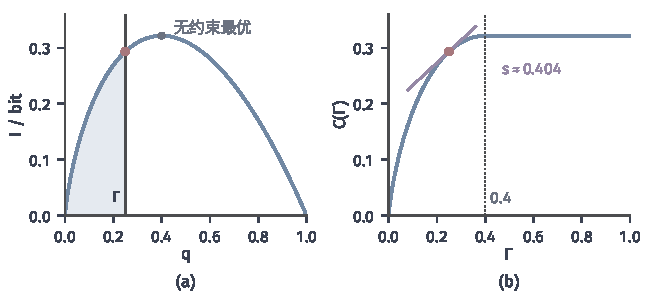
\includegraphics[width=110mm]{figures/07-probability/06-channel-coding/matplotlib/dcc-cost-capacity/figure.pdf}
 \caption{Z信道在成本$c(0)=0$、$c(1)=1$下的容量—成本函数。(a) 互信息$I(q)=h_2(q/2)-q$，浅蓝区域是预算$\Gamma=0.25$允许的输入$q\leq\Gamma$，红点为约束下的最优点，灰点为无约束最优点$q=0.4$；(b) $C(\Gamma)$，紫线是$\Gamma=0.25$处的切线，斜率$s\approx0.404$比特每单位成本，点线标出$\Gamma=0.4$。}
 \label{fig:dcc-cost-capacity}
\end{BookInlineFigure}

\paragraph{Lagrange乘子：预算的边际价值}
图~\ref{fig:dcc-cost-capacity}(b)中切线的斜率回答“再多给一单位预算，容量能增加多少”。把约束用乘子$s\geq0$并入目标，考虑
\begin{equation}
 \max_{q\in\Delta_{\mathcal{X}}}\Bigl[I(q)-s\sum_xq(x)c(x)\Bigr]+s\Gamma .
 \label{eq:dcc-lagrangian}
\end{equation}
对每个$s\geq0$与每个可行的$q$，被减去的$s(\sum_xq(x)c(x)-\Gamma)$非正，所以$I(q)$不超过式~\eqref{eq:dcc-lagrangian}；对可行的$q$取最大值，得到
\begin{equation}
 C(\Gamma)\leq\max_{q}\Bigl[I(q)-s\sum_xq(x)c(x)\Bigr]+s\Gamma\qquad\text{对每个}\ s\geq0 .
 \label{eq:dcc-weak-duality}
\end{equation}
这是弱对偶。$\Gamma>c_{\min}$时，集中在最小成本符号上的分布严格满足预算，目标是凹函数，约束是线性的，于是强对偶成立：式~\eqref{eq:dcc-weak-duality}右边对$s$的最小值等于$C(\Gamma)$，达到最小值的$s$是$C$在$\Gamma$处的切线斜率（$C$在该点可微时）。凸优化对偶的一般理论可参考\BookChapterRef{chap:duality}{卷五第18章“对偶问题”}。

固定$s$后，式~\eqref{eq:dcc-lagrangian}中的最大化与定理~\ref{thm:dcc-kkt}的问题相同，只是线性项多了$-s\sum_xq(x)c(x)$。在定理~\ref{thm:dcc-kkt}必要性的求导中，这一项沿$q_t=(1-t)q^{*}+t\delta_{x'}$的右导数是$-s\bigl(c(x')-\sum_xq^{*}(x)c(x)\bigr)$，充分性部分的上界也照样成立。所以最优条件变为：存在常数$c'$，使
\begin{equation}
 \begin{aligned}
 D_{\mathrm{KL}}(W_x\Vert p^{*})-s\,c(x)&=c'\quad\text{若}\ q^{*}(x)>0 ,\\
 D_{\mathrm{KL}}(W_x\Vert p^{*})-s\,c(x)&\leq c'\quad\text{若}\ q^{*}(x)=0 .
 \end{aligned}
 \label{eq:dcc-kkt-cost}
\end{equation}
读法是：每个输入的信息贡献扣去它按“影子价格”$s$折算的成本后，被使用的输入应当一样划算。

在Z信道$\Gamma=0.25$处核验。斜率为
\[
 s=I'(0.25)=\frac12\log_2\frac{2-0.25}{0.25}-1=\frac12\log_27-1\approx0.4037 .
\]
输出分布$p^{*}=(\tfrac78,\tfrac18)$，两行的散度为
\[
 \begin{aligned}
 D_{\mathrm{KL}}(W_0\Vert p^{*})&=\log_2\frac87\approx0.1926 ,\\
 D_{\mathrm{KL}}(W_1\Vert p^{*})&=\frac12\log_2\frac47+\frac12\log_24=\frac12\log_2\frac{16}7\approx0.5963 .
 \end{aligned}
\]
扣去成本后，$0.1926-0=0.1926$，$0.5963-0.4037=0.1926$，两者相等；并且$C(\Gamma)-s\Gamma=0.2936-0.1009=0.1927$，与舍入误差内一致。精确地，
\[
 \frac12\log_2\frac{16}7-\Bigl(\frac12\log_27-1\Bigr)=3-\log_27=\log_2\frac87 .
\]

\paragraph{期望约束与逐条预算}
式~\eqref{eq:dcc-capacity-cost}约束的是输入分布的期望成本，它是对单个随机符号的设计要求；式~\eqref{eq:dcc-codeword-budget}约束的是每一条具体码字的成本总和。按期望成本恰为$\Gamma$的分布独立抽取码字，大约一半码字会超出预算。两者之间的联系需要论证，这是下一小节的内容。

\subsection{满足预算的编码}
\label{sec:dcc-cost-coding}

下面的定理说明，在逐条预算下，$C(\Gamma)$正是可靠传输的速率极限。

\begin{theorem}[成本约束下的编码定理]
\label{thm:dcc-cost-coding}
设$\Gamma>c_{\min}$。在每条码字满足式~\eqref{eq:dcc-codeword-budget}的要求下，每个$R<C(\Gamma)$都可达，并且可以要求最大错误概率趋于零；每个$R>C(\Gamma)$都不可达。
\end{theorem}

\begin{proof}
可达性。设$R<C(\Gamma)$。由定理~\ref{thm:dcc-capacity-cost}，$C$在$\Gamma$处连续，可以取$\Gamma'\in(c_{\min},\Gamma)$使$C(\Gamma')>R$。取$q'$使$\sum_xq'(x)c(x)\leq\Gamma'$且$I(q')=C(\Gamma')$。这一步为预算留出了余量$\Gamma-\Gamma'>0$。

按$q'$抽取随机码本，用联合典型解码。定理~\ref{thm:dcc-achievability}的证明对任何满足$I(q)>R$的输入分布都成立，所以存在$\delta_n\to0$，使每条消息的期望错误$\mathbb{E}[\lambda_m]\leq\delta_n$。另一方面，记$B_m$为第$m$条码字超出预算的事件。码字的平均成本$\frac1n\sum_ic(\mathsf{X}_i(m))$是$n$个独立同分布、取值有界的变量的平均，均值不超过$\Gamma'<\Gamma$，由弱大数律，
\[
 \beta_n=\mathbb{P}(B_m)\leq\mathbb{P}\Bigl(\frac1n\sum_{i=1}^{n}c(\mathsf{X}_i(m))-\Gamma'>\Gamma-\Gamma'\Bigr)\to0 .
\]
于是随机码本满足
\[
 \mathbb{E}\Bigl[P_{\mathrm{e}}+\frac1M\sum_{m=1}^{M}\mathbf{1}_{B_m}\Bigr]\leq\delta_n+\beta_n=:\eta_n ,
\]
存在一个具体码本，其平均错误概率与超支码字的比例之和不超过$\eta_n$。

删去两类消息：条件错误概率超过$4\eta_n$的消息，按第~\ref{sec:dcc-max-error}小节的计数少于$M/4$条；超支的消息，至多$\eta_nM$条，$n$足够大使$\eta_n\leq\tfrac14$时不超过$M/4$条。保留的消息至少有$M/2$条，每条码字都守住预算，最大错误概率不超过$4\eta_n$，码率损失不超过$1/n$。与引理~\ref{lem:dcc-expurgation}后的论证一样，先用$R<R'<C(\Gamma)$构造码列再删除，就得到码率不低于$R$的码列。

逆定理。设一列满足逐条预算的码有$M\geq2^{nR}$且$P_{\mathrm{e}}\to0$。消息均匀，记第$i$个输入符号$X_i$的分布为$q_i$，期望成本$\Gamma_i=\mathbb{E}[c(X_i)]$。逆定理证明中的Fano与数据处理步骤不变，引理~\ref{lem:dcc-block-bound}的第一个不等式给出
\[
 \log_2M\leq1+P_{\mathrm{e}}\log_2M+\sum_{i=1}^{n}I(X_i;Y_i)\leq1+P_{\mathrm{e}}\log_2M+\sum_{i=1}^{n}C(\Gamma_i) .
\]
由$C$的凹性（Jensen不等式）与单调性，
\[
 \frac1n\sum_{i=1}^{n}C(\Gamma_i)\leq C\Bigl(\frac1n\sum_{i=1}^{n}\Gamma_i\Bigr)\leq C(\Gamma) ,
\]
最后一步因为
\[
 \frac1n\sum_{i=1}^{n}\Gamma_i=\mathbb{E}\Bigl[\frac1n\sum_{i=1}^{n}c(X_i)\Bigr]\leq\Gamma :
\]
每条码字的平均成本都不超过$\Gamma$，对消息平均后也不超过。于是$P_{\mathrm{e}}\geq1-(nC(\Gamma)+1)/\log_2M$，与定理~\ref{thm:dcc-converse}同理，$R>C(\Gamma)$不可达。
\end{proof}

可达性证明中的两个余量各有作用。码率余量$C(\Gamma')-R>0$控制解码错误，与无约束时相同；预算余量$\Gamma-\Gamma'>0$让大数律把码字成本压在预算以内。若直接用期望成本恰为$\Gamma$的分布，超支的码字比例不趋于零，删除会损失一个固定比例的消息。图~\ref{fig:dcc-codeword-cost}画出Z信道上$q'=0.22$、$\Gamma=0.25$时单条随机码字的平均成本分布：$n=50$时超支的概率约为$0.296$，$n=400$时降到约$0.067$，并继续趋于零。所用输入的互信息为$C(0.22)=h_2(0.11)-0.22\approx0.280$，略低于$C(0.25)=0.294$，这是为预算余量付出的码率。

\begin{BookInlineFigure}
 \centering
 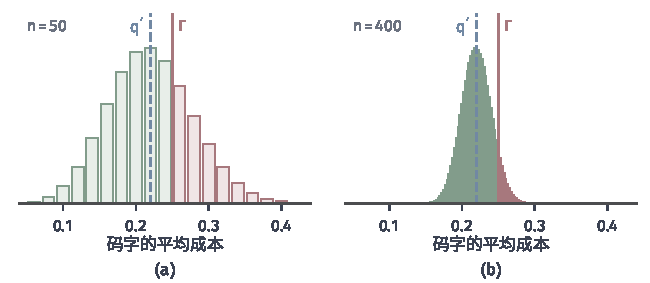
\includegraphics[width=110mm]{figures/07-probability/06-channel-coding/matplotlib/dcc-codeword-cost/figure.pdf}
 \caption{Z信道、成本$c(1)=1$，码字符号独立地以概率$q'=0.22$取$1$时，单条码字的平均成本$K/n$（$K\sim\mathrm{Bin}(n,0.22)$）的精确分布。蓝色虚线为$q'$，红线为预算$\Gamma=0.25$，红色柱为超出预算的码字。(a) $n=50$；(b) $n=400$。}
 \label{fig:dcc-codeword-cost}
\end{BookInlineFigure}

逆定理只用到了“对消息平均的成本不超过$\Gamma$”。所以即使放宽要求，只限制各码字成本的平均值，容量也不会超过$C(\Gamma)$；而可达性给出的码满足更严格的逐条预算。两种口径给出同一个容量。

\paragraph{预算等于最小成本}
$\Gamma=c_{\min}$时，余量论证无法进行，因为不存在$\Gamma'<\Gamma$。但此时约束本身变得简单：每个$c(x_i)\geq c_{\min}$，总和不超过$nc_{\min}$只能让每一项都等于$c_{\min}$。所以码字只能使用集合$\mathcal{X}_0=\{x:c(x)=c_{\min}\}$中的符号，成本约束自动满足。这相当于把输入字母表缩小为$\mathcal{X}_0$、转移矩阵只保留相应的行，对这个新信道应用无约束的定理~\ref{thm:dcc-coding-theorem}，容量为$\max\{I(q):q\ \text{支撑在}\ \mathcal{X}_0\ \text{上}\}$。这恰好等于$C(c_{\min})$，因为平均成本等于$c_{\min}$的分布正是支撑在$\mathcal{X}_0$上的分布。在Z信道中$\mathcal{X}_0=\{0\}$，只能发送$0$，容量为零。
